\documentclass[conference]{IEEEtran}
\IEEEoverridecommandlockouts

\usepackage{cite}
\usepackage{amsmath,amssymb,amsfonts}
\usepackage{graphicx}
\usepackage{booktabs}
\usepackage{tikz}
\usetikzlibrary{arrows.meta,positioning}
\usepackage[hyphens]{url}
\usepackage[hidelinks]{hyperref}

\begin{document}

\title{Learned Acoustic Signalling for Occlusion-Aware\\
Robot Navigation in Dense Crowds}

\author{\IEEEauthorblockN{Ashwinder Pal Singh}
\IEEEauthorblockA{Dept.\ of Mechanical Engineering\\
Thapar Institute of Engineering and Technology\\
Patiala, India\\
asingh47\_be23@thapar.edu}
\IEEEauthorblockA{\textit{Lab project report: Edge AI and Robotics: Reinforcement Learning}}}

\maketitle

% =============================================================================
\begin{abstract}
Can a crowd-navigation robot use sound both to clear its path and to locate people it cannot
see? We give a deep reinforcement learning policy a learned acoustic action: it can beep, nearby
pedestrians may step aside and reply, and the robot hears the replies as noisy range and bearing
estimates, including from pedestrians hidden behind obstacles. The policy builds on HEIGHT, a
heterogeneous graph-transformer navigation policy, extended with trajectory prediction and
variational occlusion inference, and is trained with proximal policy optimisation in a PyBullet
simulation with a differential-drive TurtleBot2 among ORCA pedestrians. In a matched-budget
ablation evaluated on $3{,}500$ episodes per arm, the beep raises success by about one point at
the nominal crowd density (not significant on one test set) and by $2.5$ points with $10$--$14$
pedestrians ($p=0.008$). Hearing the replies localises $2.6$ hidden pedestrians per episode but
adds nothing measurable to success over beeping alone: the benefit comes from clearing the path,
not from sensing. It also depends on a simulator assumption we state explicitly, that
pedestrians who cannot perceive the robot still obey its beep. We report the design, the reward,
the failures we found along the way, and the size of each model.
\end{abstract}

% =============================================================================
\section{Introduction}

Picture a delivery robot in a hospital corridor at shift change. Most people see it and
step aside; one nurse reading a chart does not, and the robot is struck from the side. The
scenario contains the central difficulty of social navigation: the robot's safety depends on
behaviour it does not control, and on people it cannot always see.

This project gives a learned navigation policy a way to \emph{act on the crowd}. Starting from
a platform built on HEIGHT~\cite{height}, a current reference architecture for crowd navigation,
extended with a module that anticipates where each pedestrian will be over the next half
second~\cite{intention} and a module that infers pedestrians hidden behind obstacles~\cite{pas},
we gave the policy a beep, learned jointly with its motion. Nearby pedestrians may answer by
stepping aside and by replying, so that the robot can also localise people it cannot see by ear.

\textbf{Objectives.} (i) Design an acoustic signalling and listening extension and train it with
deep reinforcement learning; (ii) separate its two possible mechanisms, clearing the path and
sensing hidden pedestrians, with matched-budget ablations; (iii) evaluate every variant at a
statistical power high enough to detect a two-point change in success, including in denser
crowds and among more obstacles; (iv) report model size and training compute, which matter for
running such a policy on an on-board computer. The base platform's own evaluation against HEIGHT
is the subject of a companion study~\cite{companion}; here it serves as the matched baseline.

The results were mostly negative, and we report them in full. Section~\ref{sec:formulation}
states the learning problem, Sections~\ref{sec:system} and~\ref{sec:acoustic} describe the
system and the acoustic extension, Section~\ref{sec:eval} reports the evaluation, and
Sections~\ref{sec:discussion} and~\ref{sec:limitations} discuss what the results do and do not
show.

% =============================================================================
\section{Background}

\textbf{Crowd navigation with deep RL.} A robot must reach a goal through a space containing
moving pedestrians and static obstacles. Learned approaches encode the scene as a
graph---robot, humans and obstacles as nodes, interactions as edges---and train a policy by
reinforcement learning in simulation~\cite{dsrnn,intention,height}. HEIGHT~\cite{height}
distinguishes human and obstacle nodes and applies separate attention networks to robot-human
and human-human edges.

\textbf{Pedestrian simulation.} Pedestrians follow ORCA~\cite{orca}, a reciprocal
velocity-obstacle method: each agent selects a velocity that avoids every agent it observes.
HEIGHT's configuration sets \texttt{robot.visible\_prob}\,$=0.2$: each moving pedestrian has a
$20\%$ chance of including the robot in its ORCA observation, and standing pedestrians never
do, so averaged over the crowd-size distribution $17.6\%$ of pedestrians can perceive the robot.
We keep this benchmark setting throughout.

\textbf{Occlusion inference.} Mun \emph{et al.}~\cite{pas} train two variational encoders: a
teacher on ground-truth occupancy and a student on partial lidar occupancy, with a distillation
loss pulling the student's latent toward the teacher's. At inference only the student runs.

\textbf{Acoustic signalling.} Nishimura and Yonetani~\cite{l2b} let a robot learn when to emit
an audible cue that makes nearby pedestrians yield, trading safety against efficiency. Our beep
model follows theirs; the listening channel, in which pedestrians' replies are used as a
sensor, is our addition.

% =============================================================================
\section{Learning Problem}
\label{sec:formulation}

We treat navigation as a partially observed Markov decision process with time step
$\Delta t=0.1$\,s and a $50$\,s time limit in a $12\times12$\,m arena with $5$--$9$ pedestrians and
$8$--$12$ rectangular obstacles per episode.

\textbf{Observation.} The robot state $[p_x,p_y,g_x,g_y,\theta]$; for each detected pedestrian
its position and velocity, extended by predicted future positions (Sec.~\ref{sec:system}); a
$180$-ray lidar scan of static obstacles; and an occupancy grid of visible pedestrians for
occlusion inference. Pedestrians hidden behind obstacles or other pedestrians are not observed.

\textbf{Actions.} Nine discrete changes of commanded linear and angular velocity,
$(\Delta v,\Delta\omega)\in\{-0.05,0,0.05\}\,\mathrm{m/s}\times\{-0.1,0,0.1\}\,\mathrm{rad/s}$, with
$v\le0.5$\,m/s. With the acoustic extension the action space doubles to $18$: each motion
with or without a beep.

\textbf{Reward.}
\begin{equation}
r_t = r_{\text{goal}} + r_{\text{coll}} + r_{\text{ps}} + \big(\phi(s_{t+1})-\phi(s_t)\big)
      - 0.05\,\omega_t^2 - 0.025 + r_{\text{ac}},
\end{equation}
with $r_{\text{goal}}=+20$ on arrival, $r_{\text{coll}}=-20$ on collision, $r_{\text{ps}}$ a
proportional penalty for entering a $0.25$\,m personal-space zone around any pedestrian,
$\phi$ a potential that rewards progress toward the goal, a spinning penalty and a per-step
cost. The acoustic term $r_{\text{ac}}$ is defined in Sec.~\ref{sec:acoustic}.

\textbf{Algorithm.} Proximal policy optimisation~\cite{ppo} with a shared recurrent
actor-critic: $28$ parallel environments, $30$ steps per rollout, learning rate
$5\times10^{-5}$ with linear decay, $\gamma=0.99$, GAE $\lambda=0.95$, clip $0.2$, entropy
coefficient $0.01$.

% =============================================================================
\section{System}
\label{sec:system}

\subsection{Architecture}
Fig.~\ref{fig:arch} shows the pipeline. Each detected pedestrian contributes
$[p_x,p_y,v_x,v_y]$ extended by five predicted future positions (14 values). The lidar scan is
encoded by HEIGHT's 1D CNN. For occlusion inference a robot-centred $10\times10$\,m occupancy
grid of the pedestrians visible to a second $360^\circ$ ray scan, with cells hidden behind the
first object on each ray marked unknown, enters the PaS student encoder, whose 256-dimensional
latent is appended to the robot state to form a 261-dimensional robot node. HEIGHT's attention
layers relate the robot node to the pedestrian nodes, and its recurrent robot-node network
combines the result with the obstacle features to select the action.

\begin{figure}[t]
\centering
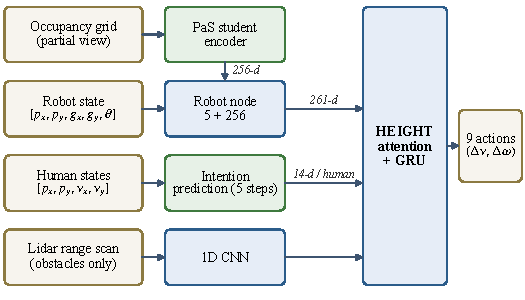
\includegraphics[width=\columnwidth]{fig_architecture}
\caption{System pipeline. Green blocks are our additions; blue blocks are HEIGHT's and
unchanged, except that the robot node also carries the 256-dimensional occlusion latent.
Obstacles reach the policy only through the lidar range scan.}
\label{fig:arch}
\end{figure}

\subsection{Intention prediction}
Human nodes are extended with five predicted future positions at $0.1$\,s intervals. The
predictions come from rolling each pedestrian's own ORCA policy and goal forward in the
simulator without the robot (\texttt{sim.predict\_method\,=\,'truth'}), holding each
pedestrian's current goal fixed. \textbf{This is privileged simulator state, not something a
deployed robot could compute.} We adopted it as a near-best case for what a learned predictor
could contribute; HEIGHT's released configuration uses no prediction. A learned predictor is
scaffolded in the code but was not used for the results here.

\subsection{Occlusion inference}
We pre-train the teacher on ground-truth occupancy grids collected from 1{,}000 training
episodes driven by uniformly random actions, then freeze its weights. The student is trained
from scratch jointly with the policy under the distillation loss (coefficient $1.0$). We audited
the inference path and confirmed that the teacher is never called at test time; the student
sees only the partial grid. The teacher is therefore not part of the deployed model.

\subsection{Training}
The combined policy (Stage~2) trained in two segments: $76$\,M steps from scratch, then a
relaunch from that checkpoint which reset the optimiser, the learning-rate schedule and the
step counter and ran a full $300$\,M-step schedule. Every arm evaluated here adds a further
$50$\,M-step fine-tune to that shared checkpoint (Sec.~\ref{sec:acoustic}), for approximately
$426$\,M environment steps in total. On a 40\,GB MIG partition of an NVIDIA H100,
at ${\sim}829$ environment steps per second, a $50$\,M-step fine-tune took roughly $17$ hours.

\subsection{Engineering notes}
Two issues consumed substantial time and are worth recording. First, an early version of the
observation code exposed the positions of occluded pedestrians to the policy and inflated its
success until an audit of the observation pipeline found it (Sec.~\ref{sec:acoustic}). Second,
Gym wrappers block access to underscore-prefixed attributes, and our use of \texttt{getattr} with a default value
silently masked a metric-reporting failure. It surfaced only because we log a standard
deviation for every metric: a counter with zero variance over $3{,}500$ episodes is a bug, not a
result.

% =============================================================================
\section{Acoustic Extension}
\label{sec:acoustic}

\begin{figure}[t]
\centering
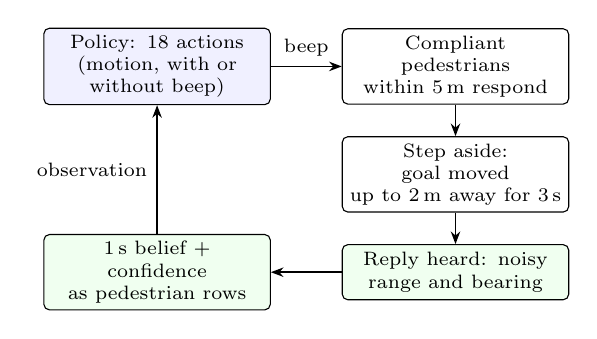
\begin{tikzpicture}[font=\scriptsize, node distance=4mm and 9mm,
  box/.style={draw, rounded corners=2pt, align=center, inner sep=2.5pt, minimum height=7mm, text width=27mm},
  arr/.style={-{Stealth[length=1.6mm]}, semithick}]
\node[box, fill=blue!6] (pol) {Policy: 18 actions\\(motion, with or without beep)};
\node[box, right=of pol] (ped) {Compliant pedestrians\\within 5\,m respond};
\node[box, below=of ped] (move) {Step aside: goal moved\\up to 2\,m away for 3\,s};
\node[box, below=of move, fill=green!6] (hear) {Reply heard: noisy\\range and bearing};
\node[box, left=of hear, fill=green!6] (bel) {1\,s belief + confidence\\as pedestrian rows};
\draw[arr] (pol) -- node[above]{beep} (ped);
\draw[arr] (ped) -- (move);
\draw[arr] (move) -- (hear);
\draw[arr] (hear) -- (bel);
\draw[arr] (bel) -- node[left, align=right]{observation} (pol);
\end{tikzpicture}
\caption{The acoustic extension. The beep can clear a path (right) and, through pedestrians'
replies, act as a sensor for people the robot cannot see (left, green). Ablations switch off
the reply channel (``beep only'') or its confidence feature.}
\label{fig:acoustic}
\end{figure}

\textbf{Beep.} When the policy chooses a beep (at most once every $2$\,s), every pedestrian
within $5$\,m receives a signal of strength $s(d)=\exp(-d^2/2\sigma^2)$, $\sigma=3$\,m. Each
pedestrian is marked \emph{compliant} at the start of an episode with probability $0.8$; a
compliant pedestrian answers a given beep with probability $0.8\,s(d)$. After a $0.2$\,s delay
it moves its goal up to $2s(d)$\,m directly away from the robot for $3$\,s, then returns to its
original goal over $1$\,s (Fig.~\ref{fig:acoustic}).

\textbf{Listening.} A responding pedestrian also replies. Within $8$\,m the robot obtains a
range and bearing fix with noise $\sigma_r=0.4$\,m and $\sigma_\theta=0.12$\,rad, both multiplied
by $2.5$ when the speaker is occluded, since diffraction around an obstacle degrades
localisation. Fixes over the $0.5$\,s reply are averaged, stored in world coordinates and kept
for $1$\,s. A pedestrian the robot cannot see but has heard enters the policy as an extra
pedestrian row. Every row carries a confidence feature, $1$ for a visual detection and a value
that decays with the fix's expected error and age for an audio estimate.

\textbf{Reward.} $r_{\text{ac}} = -0.1$ for each beep, plus $0.05$ for each previously
untriggered pedestrian the robot cannot see who is triggered by it, so the information bonus
cannot be farmed by beeping at people already in view.

\textbf{Training arms.} All arms start from the shared Stage~2 checkpoint and are fine-tuned
for $50$\,M steps with the same seed; only the acoustic switches differ. New input and output
weights (the beep flag, the confidence column and the nine beep actions) are initialised fresh.
The arms are: \emph{no acoustics} (the matched baseline), \emph{beep only} (no replies),
\emph{beep + listening} (full), and \emph{beep + listening without the confidence feature}. All
keep the privileged futures.

\textbf{Development history.} Earlier versions failed in instructive ways. In the first, the
audio rows carried the exact positions of hidden pedestrians---a wall-hack that inflated success
until an audit of the observation pipeline found it---and the information reward never fired,
because the action was remapped to a motion before the reward checked for a beep; its results
were discarded. With both fixed, a version whose audio fixes lasted only the $0.5$\,s of a reply
reached $90\%$ success on $500$ test episodes. Holding each fix for $3$\,s without a confidence
feature dropped success to $77\%$, with $23\%$ collisions: with no motion model, a frozen
estimate drifts by up to $1.5$\,m in $3$\,s, so the robot avoided ghosts and hit real obstacles.
The final version holds fixes for $1$\,s, which caps the drift near the fix error, and adds the
confidence feature ($90\%$ on the same $500$ episodes). These $n=500$ figures are development
measurements only; the evaluation below uses $3{,}500$ episodes per arm.

% =============================================================================
\section{Evaluation}
\label{sec:eval}

\subsection{Protocol}
All rates are over $n=3{,}500$ test episodes, which gives roughly 76\% power to detect a
2-point difference in success between two fixed checkpoints at $\alpha=0.05$; the
conventional $n=500$ has roughly 17\% power for the same effect. The primary comparison is
between arms that share the base checkpoint and training budget and differ only in the acoustic
switches. HEIGHT's released checkpoint, evaluated in our codebase with our modules disabled, is
shown for reference. Success contrasts use the pooled two-proportion $z$ test with Wald $95\%$
intervals. Because this report makes thirteen binary comparisons, we treat $p<0.004$
(Bonferroni) as the conservative bar for any single one.

\textbf{Base platform.} Without acoustics, the platform scores $88.54\%$ against $88.03\%$ for
HEIGHT's released checkpoint on the same test scenes ($+0.51$ points, $p=0.50$): no detectable
difference. Its full evaluation against HEIGHT is reported in the companion study~\cite{companion}
and not repeated here.

\subsection{Acoustic ablation}
\begin{table*}[t]
\caption{Acoustic ablation at the nominal setting, $n=3{,}500$ episodes per row. All ``Ours''
rows are the same $50$\,M-step fine-tune from one shared checkpoint with privileged futures,
differing only in the acoustic switches; the first two rows are reference rows from the
companion study~\cite{companion}. Collision and timeout columns are episode counts.
Navigation time is over successful episodes only. ``Heard'' counts hidden pedestrians
localised by their replies.}
\label{tab:acoustic}
\centering
\setlength{\tabcolsep}{4.5pt}
\begin{tabular}{lcccccccc}
\toprule
Arm & Success (\%) & Pedestrian & Obstacle/wall & Timeout & Nav.\ time (s) & Beeps/episode & Heard/episode & Intrusion (\%) \\
\midrule
HEIGHT (released) & 88.03 & 358 & 59 & 2 & $18.07\pm4.36$ & -- & -- & 5.66 \\
Ours, no acoustics & 88.54 & 336 & 56 & 9 & $18.21\pm4.41$ & 0 & 0 & 4.75 \\
Ours, beep only & 89.49 & 278 & 84 & 6 & $17.57\pm4.27$ & 5.06 & 0 & 4.22 \\
Ours, beep + listening & 89.60 & 293 & 69 & 2 & $17.60\pm4.09$ & 7.62 & 2.57 & 4.36 \\
\quad without confidence feature & 88.57 & 318 & 76 & 6 & $17.40\pm3.91$ & 6.58 & 2.35 & 4.07 \\
\bottomrule
\end{tabular}
\end{table*}

\begin{figure*}[t]
\centering
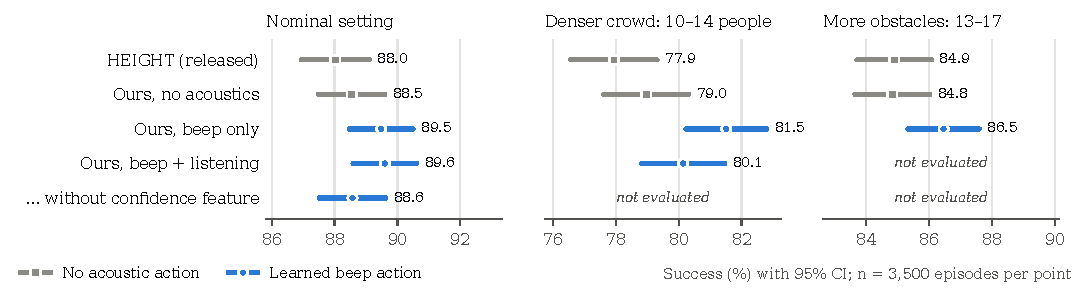
\includegraphics[width=\textwidth]{fig_results}
\caption{Success with $95\%$ intervals for every evaluated arm at the nominal setting and in
the two harder settings. Each point is one checkpoint evaluated on $3{,}500$ episodes; all
policies were trained at the nominal setting.}
\label{fig:results}
\end{figure*}

Table~\ref{tab:acoustic} and Fig.~\ref{fig:results} give the matched-budget comparison. Against
the same fine-tune without acoustics, beeping raises success by $+0.94$ points
($[-0.52,+2.41]$, $p=0.21$), and beeping with listening by $+1.06$ points ($[-0.40,+2.52]$,
$p=0.16$); neither is significant on this test set. Listening adds $+0.11$ points over beeping
alone ($p=0.88$), and removing the confidence feature costs $1.03$ points ($p=0.17$). The
listening channel does work as a sensor---the robot localises $2.57$ hidden pedestrians per
episode, $0.34$ per beep---but that information does not translate into measurably more
successful navigation.

We evaluated the full and no-acoustics checkpoints on two further independent sets of
$3{,}500$ test scenes. The difference was $+1.06$, $+0.40$ and $+1.71$ points on the three sets,
$+1.06$ points pooled over $10{,}500$ episodes ($[+0.21,+1.90]$, $p=0.014$). This replication is
across test scenes, not across training runs: it shows that this particular pair of checkpoints
differs, not that acoustic training reliably helps.

Beeping also shortens successful episodes by about $0.6$\,s (full: $-0.61$\,s, Welch
$t=-5.7$; beep only: $-0.64$\,s, $t=-5.8$) and lowers the intrusion ratio, as one would expect
when the pedestrians being beeped at walk away. The beep-only and full arms beep $5.1$ and $7.6$
times per episode ($2.9$ and $4.4$ times per $100$ steps).

\subsection{Denser crowds and more obstacles}
\begin{table}[t]
\caption{Out-of-distribution settings, $n=3{,}500$ each. All policies were trained with $5$--$9$
pedestrians and $8$--$12$ obstacles. Counts as in Table~\ref{tab:acoustic}.}
\label{tab:gen}
\centering
\begin{tabular}{lcccc}
\toprule
Arm & Success (\%) & Ped. & Obs./wall & Timeout \\
\midrule
\multicolumn{5}{l}{\textit{10--14 pedestrians}} \\
HEIGHT & 77.94 & 672 & 95 & 5 \\
Ours, no acoustics & 78.97 & 621 & 100 & 15 \\
Ours, beep only & 81.51 & 513 & 114 & 20 \\
Ours, beep + listening & 80.14 & 599 & 83 & 13 \\
\midrule
\multicolumn{5}{l}{\textit{13--17 obstacles}} \\
HEIGHT & 84.89 & 280 & 236 & 13 \\
Ours, no acoustics & 84.83 & 306 & 191 & 34 \\
Ours, beep only & 86.46 & 215 & 226 & 33 \\
\bottomrule
\end{tabular}
\end{table}

We tested the policies in the two harder conditions of HEIGHT's evaluation protocol: more
pedestrians and more obstacles (Table~\ref{tab:gen}). Without acoustics, the platform stays
level with HEIGHT ($+1.03$ points with more people, $p=0.30$; $-0.06$ with more obstacles,
$p=0.95$). The beep helps most where the crowd is densest: with $10$--$14$
pedestrians, beep-only is $+2.54$ points above the same policy without acoustics ($p=0.0076$)
and $+3.57$ points above HEIGHT ($[+1.69,+5.45]$, $p=2\times10^{-4}$, the only contrast in this
report that passes the Bonferroni bar). Listening again does not help: with more people the full
arm is $1.37$ points below beep-only ($p=0.15$) and collides with pedestrians more often
($+2.46$ points, $p=0.005$, short of the Bonferroni bar); we did not establish why. With more
obstacles, beep-only is $+1.63$ points above no acoustics ($p=0.052$).

\subsection{Model size and compute}
\begin{table}[t]
\caption{Model size. Trainable actor and critic parameters; the frozen PaS teacher is excluded
because it is not used at inference. The acoustic variants add a few input weights and nine
action outputs to ``Ours'' and were not counted separately.}
\label{tab:size}
\centering
\setlength{\tabcolsep}{4pt}
\begin{tabular}{lcc}
\toprule
Model & Parameters & Checkpoint (MiB) \\
\midrule
HEIGHT & 478{,}618 & 1.84 \\
Ours (prediction + occlusion) & 1{,}236{,}058 ($2.58\times$) & 9.13 \\
\bottomrule
\end{tabular}
\end{table}

Prediction and occlusion inference cost $2.58\times$ HEIGHT's parameters and $5\times$ its
checkpoint size (Table~\ref{tab:size}). Both models are small by current standards---a few
megabytes, well within the memory of an embedded GPU. Training is the dominant compute cost: each $50$\,M-step fine-tune took about
$17$\,hours on a 40\,GB partition of an H100, and the full combined recipe ran roughly $426$\,M
environment steps. We did
not measure on-board inference latency or power; that is the natural next measurement for a
deployment-oriented version of this work.

% =============================================================================
\section{Discussion}
\label{sec:discussion}

\textbf{The beep works by moving people, not by informing the robot.} Beeping alone captures
the whole benefit of the acoustic extension at every density we tested, and the listening
channel, although it localises hidden pedestrians as designed, adds nothing to success and may
cost collisions in dense crowds. The effect of the beep is path-clearing, which is the mechanism
of prior work~\cite{l2b}, not the sensing mechanism we set out to test.

\textbf{The benefit rests on a simulator assumption.} Compliance is drawn independently of
\texttt{visible\_prob}, so about $64\%$ of moving pedestrians ($0.8\times0.8$) are modelled as
unable to perceive the robot visually yet able to hear and obey its beep. That can be defended
(someone looking at a phone may still react to a sound), but the size of the gain is governed by
a compliance rate we chose rather than measured, and a sensitivity sweep over that rate is the
first experiment any follow-up should run. A beep every few seconds also has a social cost that
the reward does not price beyond a small penalty.

\textbf{Lessons for RL experiments.} The first acoustic version looked strong because of an
observation leak, not because of what it had learned. The fix for the stale-belief
version changed two settings at once, so which one mattered could not be told until a separate
arm removed the confidence feature. And at $n=500$ a two-point difference has only $17\%$ power, so none of our
development numbers could have decided anything. Evaluate at adequate power, change one variable
per run, audit the observation pipeline, and label privileged inputs in every table.

% =============================================================================
\section{Limitations}
\label{sec:limitations}

\textbf{Privileged information.} Every ``Ours'' result, including all acoustic arms, gives the
policy an ORCA forecast of each pedestrian computed from simulator state. No deployed robot has
this, and whether the acoustic results hold with a learned predictor is untested.

\textbf{One training seed per arm.} Each arm was trained once; the three-scene-set replication
varies test scenes, not training, so training-run variance is unmeasured.

\textbf{Out-of-distribution tests.} The denser settings were evaluated without retraining, on one
checkpoint per arm, and the full arm was not run with more obstacles.

\textbf{Simulated people.} Pedestrians are ORCA agents and their response to a beep is a
designed rule with a chosen compliance rate. How real people respond to a robot's sounds, and
whether they would tolerate several beeps per crossing, is untested.

\textbf{No hardware validation.} All results are in simulation; inference latency and power on
an embedded computer were not measured.

% =============================================================================
\section{Conclusion}

We gave a graph-transformer navigation policy, trained with PPO, a learned acoustic action with a
listening channel, and evaluated it in matched-budget ablations at a statistical power well above
the field's norm. The beep raised success where crowds were dense, but through path-clearing
under a compliance assumption, not through the information its echoes carried. The listening
channel worked as a sensor yet did not improve navigation. Code is available online~\cite{repo}.

\textbf{Code and data.} The repository contains the simulator, policy, training and evaluation
code, including the acoustic module (switched off by configuration in the released runs).

\textbf{Use of AI tools.} Anthropic's Claude was used to draft text and to write the code and
analyses described here, and OpenAI's Codex to check the code, data and statistics. The author
takes responsibility for the content.

% =============================================================================
\begin{thebibliography}{10}
\bibitem{height} S.~Liu \emph{et al.}, ``HEIGHT: Heterogeneous interaction graph transformer for robot navigation in crowded and constrained environments,'' \emph{IEEE Trans.\ Autom.\ Sci.\ Eng.}, 2026.
\bibitem{intention} S.~Liu \emph{et al.}, ``Intention aware robot crowd navigation with attention-based interaction graph,'' in \emph{Proc.\ IEEE Int.\ Conf.\ Robot.\ Autom.\ (ICRA)}, 2023, pp.~12015--12021.
\bibitem{pas} Y.-J.~Mun, M.~Itkina, S.~Liu, and K.~Driggs-Campbell, ``Occlusion-aware crowd navigation using people as sensors,'' in \emph{Proc.\ IEEE Int.\ Conf.\ Robot.\ Autom.\ (ICRA)}, 2023, pp.~12031--12037.
\bibitem{dsrnn} S.~Liu, P.~Chang, W.~Liang, N.~Chakraborty, and K.~Driggs-Campbell, ``Decentralized structural-RNN for robot crowd navigation with deep reinforcement learning,'' in \emph{Proc.\ IEEE Int.\ Conf.\ Robot.\ Autom.\ (ICRA)}, 2021, pp.~3517--3524.
\bibitem{orca} J.~van~den Berg, S.~J.~Guy, M.~Lin, and D.~Manocha, ``Reciprocal $n$-body collision avoidance,'' in \emph{Robotics Research}, 2011, pp.~3--19.
\bibitem{l2b} M.~Nishimura and R.~Yonetani, ``L2B: Learning to balance the safety-efficiency trade-off in interactive crowd-aware robot navigation,'' in \emph{Proc.\ IEEE/RSJ Int.\ Conf.\ Intell.\ Robots Syst.\ (IROS)}, 2020, pp.~11004--11010.
\bibitem{ppo} J.~Schulman, F.~Wolski, P.~Dhariwal, A.~Radford, and O.~Klimov, ``Proximal policy optimization algorithms,'' arXiv:1707.06347, 2017.
\bibitem{companion} A.~P.~Singh, K.~Jain, and H.~S.~Pannu, manuscript in preparation, 2026.
\bibitem{repo} A.~P.~Singh, ``Occlusion-aware social robot navigation in dense crowds,'' GitHub repository, 2026. [Online]. Available: \url{https://github.com/AshwinderPalSingh/Occlusion-Aware-Social-Robot-Navigation-in-Dense-Crowds-}
\end{thebibliography}

\end{document}
